\section{Results}
\label{sec:results}
\begin{table*}[t]
  \centering
  \small
  \setlength{\tabcolsep}{4.5pt}
  \begin{tabular}{lrrrrrrrr}
    \toprule
    \textbf{Model} & \textbf{NLP} & \textbf{BLiMP} & \textbf{Supp.} & \textbf{EWoK} & \textbf{Entity} & \textbf{PIQA} & \textbf{COMPS} & \textbf{GLUE} \\
    \midrule
    \multicolumn{9}{l}{\textit{Official baselines}} \\
    \quad GPT-2 (BabyLM 2026)          & \rNlpGtwo & \rBlimpGtwo & \rSuppGtwo & \rEwokGtwo & \rEntGtwo & \rPiqaGtwo & \rCompsGtwo & \rGlueGtwo \\
    \quad Interaction (BabyLM 2026)    & \rNlpInter & \rBlimpInter & \rSuppInter & \rEwokInter & \rEntInter & \rPiqaInter & \rCompsInter & \rGlueInter \\
    \midrule
    \multicolumn{9}{l}{\textit{Other Strict-Small submissions (task-complete, ranked above ours)}} \\
    \quad BabySteps-MurphysLaw (rank 1) & \textbf{\rNlpBaby} & \rBlimpBaby & \rSuppBaby & \rEwokBaby & \rEntBaby & \rPiqaBaby & \rCompsBaby & \textbf{\rGlueBaby} \\
    \quad wwm\_curriculum (rank 2)      & \rNlpWwm & \rBlimpWwm & \rSuppWwm & \textbf{\rEwokWwm} & \textbf{\rEntWwm} & \rPiqaWwm & \rCompsWwm & \rGlueWwm \\
    \quad RecGPT-10M (rank 3)           & \rNlpRec & \textbf{\rBlimpRec} & \rSuppRec & \rEwokRec & \rEntRec & \textbf{\rPiqaRec} & \textbf{\rCompsRec} & \rGlueRec \\
    \midrule
    \multicolumn{9}{l}{\textit{Ours}} \\
    \quad GPT-BERT (\rEpochs\,ep)       & \rNlpBase  & \rBlimpBase  & \rSuppBase  & \rEwokBase  & \rEntBase  & \rPiqaBase  & \rCompsBase  & \rGlueBase  \\
    \quad \textbf{+ \MPO{}} (\rDpoEpochs\,ep) & \rNlpDpo & \rBlimpDpo & \textbf{\rSuppDpo} & \rEwokDpo & \rEntDpo & \rPiqaDpo & \rCompsDpo & \rGlueDpo \\
    \bottomrule
  \end{tabular}
  \caption{\textbf{Main results on the official BabyLM~2026 Strict-Small
  metrics} (Overall NLP average and its seven task components; AoA and reading
  omitted, since AoA rounds to zero for nearly every submission under the
  corrected scorer, the GPT-2 baseline at \rAoaGtwo{} being the exception).
  Entity Tracking is the bias-filtered version; PIQA is
  GlobalPIQA. Comparison rows are the task-complete entries ranked above
  ours on the
  live leaderboard (fetched \rBoardFetch{}, \rFieldSize{} entries;
  submissions that have
  not rerun the new Entity/PIQA tasks are omitted). Our entries rank
  \rRankDpo{} and \rRankBase{}; \textbf{bold} marks the
  best value per column among the tabulated entries.
  \MPO{} improves over our fully-trained baseline on five of seven columns while
  using \rDpoEpochs{} rather than \rEpochs{} epochs.}
  \label{tab:main}
\end{table*}


\subsection{A Controlled Study of In-Training Interventions}
\label{sec:search}

\begin{table}[t]
  \centering
  \footnotesize
  \setlength{\tabcolsep}{3pt}
  \begin{tabular}{llrr}
    \toprule
    \textbf{Intervention} & \textbf{Site} & \textbf{BLiMP} & \textbf{Suppl.} \\
    \midrule
    Baseline hybrid                & ---        & \rFastBase   & \rFastSuppBase \\
    \midrule
    Contrastive grammat.$^{\dagger}$ & objective  & \rLevContrB  & \rLevContrS \\
    Span masking                   & objective  & \rLevSpanB   & \rLevSpanS  \\
    Muon optimizer             & optimizer  & \rLevMuonB   & \rLevMuonS  \\
    Checkpoint averaging                       & weights    & \rLevSoupB   & \rFastSuppBase \\
    Adaptive masking                   & masking    & \rLevAdaptB  & \rLevAdaptS \\
    Selective LM                        & token loss & \rLevSlmB    & \rLevSlmS   \\
    Morph.-aware tokenization                      & tokenizer  & \rLevMorphB  & \rLevMorphS \\
    \midrule
    \MPO{} (\S\ref{sec:method})    & post-training & \textbf{70.24} & \textbf{65.60}$^{*}$ \\
    \bottomrule
  \end{tabular}
  \caption{\textbf{Eight interventions, one improvement.} Fast BLiMP and BLiMP
  Supplement under an identical budget, recipe, and seed; every intervention
  changes
  one component relative to the baseline hybrid. $^{\dagger}$Contrastive
  training crashed at 77M words and is compared at the matched 70M checkpoint
  (reference 70.13/65.60). $^{*}$Supplement varies with seed on this
  50-item-per-subtask
  fast set (\S\ref{sec:results-mpo}). A planned self-distillation
  intervention
  never produced a comparable run: three resident fp32 teachers exceed 16\,GB,
  which we report as a hardware exclusion rather than a result.}
  \label{tab:levers}
\end{table}


The principles of \S\ref{sec:method} make falsifiable predictions: if timing
binds, no intervention injected \emph{during} acquisition should surpass the
baseline; if preservation binds,
unanchored signals should damage $\mathcal{F}$ before anything else; and if
configuration sensitivity is as severe as the alignment principle assumes,
gains imported from neighboring setups should not transfer. We test all three
with a controlled study of seven in-training interventions spanning the
sites where signal enters the update rule (objective, optimizer, weights,
masking policy, token-level loss, tokenizer), each run holding budget, data
order, and seed fixed while changing one component, and each gated by the
same
fast BLiMP-and-supplement evaluation. An eighth planned intervention,
ensemble
self-distillation, was excluded by hardware constraints
(Table~\ref{tab:levers}). The scope is deliberate: the predictions
concern how the update rule reshapes the model, so the study varies that
rule while holding the data stream fixed; data-side methods such as
curricula lie outside it, and under a corpus traversed ten times, replay
is the default rather than a distinct option.
Table~\ref{tab:levers}
collects the outcomes, and they fall where the principles predict. No
in-training intervention improves on the baseline.

The objective-side interventions regress most severely. The contrastive
grammaticality loss
costs seven BLiMP points while its own auxiliary loss collapses toward zero,
a shortcut at the task's expense; span masking, a harder
reconstruction task per epoch, underfits the fixed budget. Muon degrades
both, a higher training loss than AdamW at equal words seen and weaker
transfer besides, a mismatch with this budget-bound regime rather than a
verdict on the optimizer. Averaging
late checkpoints has no effect; by 80M words they occupy a shared basin. Adaptive
masking arrives with a reported one-point BLiMP gain on a DeBERTa encoder
\citep{edman2025mask} and transfers to our hybrid as a tie. Morphology-aware
tokenization arrives reporting EWoK gains of roughly twenty percent and
entity-tracking gains of roughly forty percent at this budget
\citep{bolucu2025morpheme}
and inverts under our recipe: EWoK falls below chance, to \rLevMorphEwok{}. Selective language
modeling \citep{lin2024rho,mindermann2022prioritized} holds BLiMP but gives
up seven supplement points: excess-loss selection de-weights the most
predictable text, child-directed dialogue, and with it the pragmatics the
supplement measures.

The regressions also share a structure, the preservation prediction made
visible. In Figure~\ref{fig:fragile}, four mechanistically unrelated
interventions degrade the same two filler--gap phenomena first, by 15 to 60
points, while typically gaining on easier local subtasks. Long-distance
dependencies are both the last structure acquired and the first sacrificed
when the signal is perturbed; a viable intervention must leave them
alone. Nor does greater intensity rescue a proxy, which is why
preservation requires an explicit anchor: the contrastive loss reaches
near zero as BLiMP falls, Muon fits the MLM objective harder and
generalizes worse, and \S\ref{sec:results-mpo} shows the same trade-off
within our own method. At 33M parameters and 10M words there is no spare
capacity, and a proxy pursued past the anchor's tolerance is paid in
competence.
% numbers from DPO_ABLATIONS.md + dpo_canary logs (fast eval at the step-1250 operating point)
\begin{table}[ht]
  \centering
  \small
  \setlength{\tabcolsep}{3.2pt}
  \begin{tabular}{llccrr}
    \toprule
    \textbf{Init} & \textbf{Negatives} & $\beta$ & \textbf{Seed} & \textbf{BLiMP} & \textbf{Suppl.} \\
    \midrule
    \multicolumn{4}{l}{\textit{no preference phase (baseline)}} & \rFastBase & \rFastSuppBase \\
    \midrule
    70M  & mixed & 0.1 & 42 & \textbf{70.24} & \textbf{65.60} \\
    70M  & mixed & 0.1 & 43 & 70.14 & 64.40 \\
    70M  & mixed & 0.1 & 44 & \textbf{70.28} & 63.60 \\
    30M  & mixed & 0.1 & 42 & 64.96 & 62.80 \\
    99M  & mixed & 0.1 & 42 & 70.26 & 62.40 \\
    70M  & hard  & 0.1 & 42 & 70.16 & 64.40 \\
    70M  & hard  & 0.2 & 42 & 70.14 & 64.00 \\
    \bottomrule
  \end{tabular}
  \caption{\textbf{\MPO{} ablations} (fast BLiMP / Supplement at the step-1250
  operating point). Seeds vary the entire phase, not just data order. The two
  init rows bracket the saturation checkpoint: from 99M the phase matches the
  70M-init BLiMP while spending 29M more words of budget, and from the
  pre-saturation 30M checkpoint it stays near that checkpoint's own baseline
  (\rThirtyBaseB{}/\rThirtyBaseS{}), five points below every saturated init.
  ``Hard'' reweights corruptions toward the more adversarial edit
  types; together with the larger $\beta$ it raises preference accuracy
  (0.85$\rightarrow$0.90) and lowers evaluation scores. The supplement column
  is measured on 50 items per subtask and fluctuates accordingly.}
  \label{tab:ablations}
\end{table}

Portability fares no better: the masking-policy result does not survive
the change from encoder to hybrid, and the tokenizer result inverts under
a different recipe and evaluation pipeline. At this scale results are
sensitive to interactions among architecture, recipe, and metric;
re-validation under one's own budget is a prerequisite. The study thus confirms each prediction: the region of
the design space the principles exclude, in-training injection of
unanchored signal, is empty as far as this search reaches, and the region
they license contains \MPO{}. Appendix~\ref{sec:app-mech} gives a
mechanistic reading of the shared pattern in terms of basin geometry and
gradient competition.

\subsection{\MPO{}}
\label{sec:results-mpo}
Table~\ref{tab:main} reports both submitted models on the official
Strict-Small metrics. \MPO{} improves on the fully-trained baseline in five
of seven task columns, gives back under a point on the other two (EWoK and
COMPS), ties reading (\rReadDpo{} vs.\ \rReadBase{}, both near zero), and
lifts the NLP average from \rNlpBase{} to \rNlpDpo{} at \rDpoEpochs{}
rather than
\rEpochs{} epochs ($\rDpoWords$ vs.\ $\rWordsSeen$ words seen). The two
entries place \rRankDpo{} and \rRankBase{} among
\rFieldSize{},\footnote{Model and all checkpoints are public at
\url{https://huggingface.co/Ujjwal101/ujjwal-very-bored}. Leaderboard
standings fetched \rBoardFetch{}.} We sit near the top of the field on the
BLiMP supplement; entity tracking and the world-knowledge tasks
(EWoK, GlobalPIQA) are where we trail the leaders, a gap no measurement
choice narrows. Across three seeds,
fast BLiMP holds at $\rBlimpSeedMean\pm\rBlimpSeedSd$ and, uniquely among
every intervention we tried, $\mathcal{F}$ \emph{improves}
(\emph{wh\_vs\_that\_with\_gap}
\rWhGapBase{}$\rightarrow$\rWhGapDpo{}, consistent across seeds and
configurations); the full-suite gains on entity tracking, GlobalPIQA, and
GLUE are from the submitted single-seed run (see Limitations).

The pattern across columns is inconsistent with teaching to the test. The
benchmark nearest the training signal moves least: full BLiMP gains
\rBlimpDeltaFull{}. The clear gains appear where the corruptions never
reach, dialogue pragmatics in the supplement, entity tracking, GlobalPIQA,
and finetuned GLUE, and Table~\ref{tab:ablations} shows that pushing the
proxy harder degrades the evaluation; a model exploiting the format would
show the opposite, gains only where the format matches.

The direction of the small losses follows from what the signal contains.
The corruptions manipulate structure, never facts, so the phase sharpens
sensitivity to well-formedness but teaches nothing about the world; EWoK
and COMPS contrast plausibility rather than grammar, and mass reallocated
toward well-formedness leaves such contrasts untouched or marginally
taxed. Both drops are under a point, and \S\ref{sec:diagnosis} shows world
knowledge was never acquired in the first place: nothing there for
refinement to refine.
\begin{figure}[t]
  \centering
  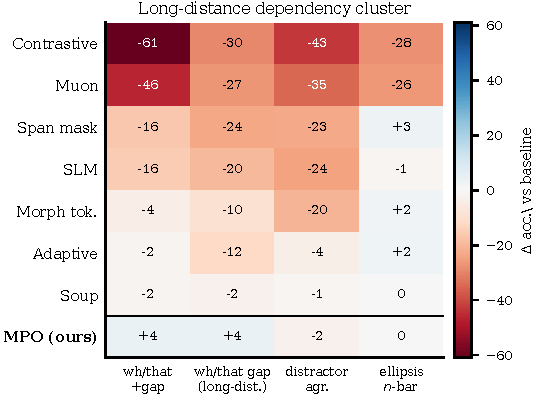
\includegraphics[width=\columnwidth]{figures/fig_fragile}
  \caption{\textbf{Every failed intervention degrades the same cluster; only
  \MPO{}
  repairs it.} Change in fast-BLiMP accuracy on the fragile long-distance
  dependency cluster $\mathcal{F}$ relative to the Phase-1 baseline, per
  intervention. Red = degraded, blue = improved. The objective- and
  optimizer-side
  interventions (Contrastive, Muon) reduce filler--gap licensing by 40--60
  points;
  \MPO{} (bottom) is the only intervention that \emph{improves} it.}
  \label{fig:fragile}
\end{figure}

\label{sec:results-ablations}
\begin{figure*}[t]
  \centering
  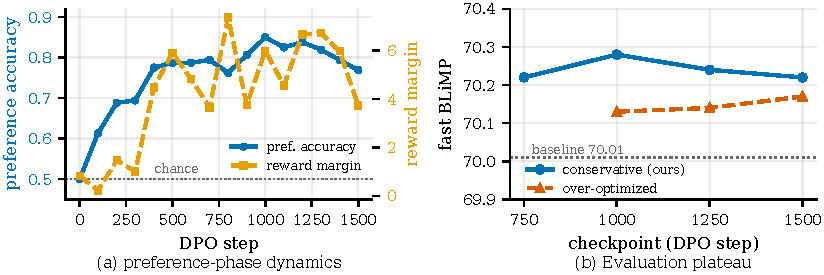
\includegraphics[width=2\columnwidth]{figures/fig_dynamics}
  \caption{\textbf{\MPO{} dynamics and the eval plateau.} (a)~Preference accuracy
  rises to $\sim\!0.85$ and the reward margin grows: the objective is learned.
  (b)~Fast BLiMP across checkpoints: the conservative run (ours, $\beta{=}\rBeta$)
  holds a plateau above the baseline, ruling out checkpoint-selection effects,
  while the over-optimized variant ($\beta{=}0.2$, harder negatives) plateaus
  below it despite higher preference accuracy.}
  \label{fig:dynamics}
\end{figure*}



Four alternative explanations could undermine the result;
Table~\ref{tab:ablations}
collects the runs that test them. \emph{Seed sensitivity.} Seeds 43 and 44
leave fast BLiMP at $\rBlimpSeedMean\pm\rBlimpSeedSd$, the $\mathcal{F}$
repair recurs in every saturation-init run, and the 50-item supplement
fluctuates as noise. \emph{Checkpoint selection.} Figure~\ref{fig:dynamics}b
shows checkpoints 750 through 1{,}500 spanning 70.22 to 70.28, a plateau.
\emph{Initialization.} The starting point matters in both directions.
From the 99M-word checkpoint the identical phase reaches \rInitFinalB{},
the same BLiMP for 29M more words; from the pre-saturation
30M checkpoint it reaches \rInitThirtyB{}, a small gain over its own
\rThirtyBaseB{} and five points short of every saturated-init run.
Refinement tracks its starting competence and substitutes for none of it;
the diagnosis identifies a causal precondition, not a descriptive
landmark. \emph{Objective strength.} Hard negatives at $\beta=\rBeta$ give
\rHardNegB{}; $\beta{=}0.2$ gives \rVtwoB{} while preference accuracy rises
from \rPrefAcc{} to \rPrefAccHard{}, the proxy improving as the evaluation
deteriorates, the \S\ref{sec:search} trade-off within our own method. The
conservative configuration is not an untuned default but the optimum here.

\subsection{Submission}
\label{sec:submission}
Both models are separate leaderboard entries, the fully trained baseline
and the \MPO{} model; each is the organizers' server-scored collation over
the complete suite with the required checkpoints, so no number in
Table~\ref{tab:main} is from our own harness. The hybrid uses the
pipeline's masked next-token (\texttt{mntp}) backend for the zero-shot
tasks and its causal backend for entity tracking and age of acquisition;
the \MPO{} entry declares its true \rDpoWords{}-word exposure against the
100M cap. The two entries hold \rRankDpo{} and \rRankBase{} among
\rFieldSize{}; the board is live but the within-submission comparison is
not, since the same \rParamsM{} model appears twice, with and without the
reallocated tail, every difference a \rDpoMinutes{}-minute phase.
